% file: sections/appendix.tex

\section{附录}

\appendix

%%%%%%%%%%%%%%%%%%%% Begin: Jupiter %%%%%%%%%%%%%%%%%%%%

%%%%%%%%%%%%%%%%%%%%
\begin{frame}{}
  \begin{cdef}[最终收敛性 (Eventual Convergence)~\ncite{Ellis:SIGMOD89}]
    当用户不再提交更新操作时, 所有 replicas 上的列表是相同的。
  \end{cdef}

  \pause
  \vspace{0.50cm}

  \begin{cdef}[强最终一致性 (Strong Eventual Consistency)~\ncite{Shapiro:SSS11}]
    如果两个 replicas 处理了同一组更新操作, 则它们的列表是相同的。
  \end{cdef}

  \pause
  \vspace{0.60cm}
  \centerline{\red{\large 对系统的\red{中间状态}缺少足够的约束}}
\end{frame}
%%%%%%%%%%%%%%%%%%%%

%%%%%%%%%%%%%%%%%%%%
\begin{frame}{}
  \centerline{\large 针对列表的操作转换函数~\ncite{Ellis:SIGMOD89}}

  \resizebox{\textwidth}{!}{
    \begin{minipage}{\textwidth}
      % file: parts/list-ot.tex

\newcommand{\ldel}{\textsc{Del}}	% List DEL
\newcommand{\lins}{\textsc{Ins}}	% List INS
\newcommand{\ldelop}[2]{\ldel\left(#1, #2\right)}  % #1: index, #2: priority
\newcommand{\linsop}[3]{\lins\left(#1, #2, #3\right)}  % #1: index, #2: element, #3: priority

%%%%%%%%%% list-ot.tex %%%%%%%%%% 
\begin{align*}
  % ins vs. ins
  OT\Big(\lins(a_1, p_1, pr_1), \lins(a_2, p_2, pr_2)\Big) &= \begin{cases}
    \lins(a_1, p_1, pr_1) 		& p_1 < p_2 \\[3pt]
    \lins(a_1, p_1 + 1, pr_1) 		& p_1 > p_2 \\[3pt]
    \textsc{NOP} 			& p_1 = p_2 \land a_1 = a_2 \\[3pt]
    \lins(a_1, p_1 + 1, pr_1) 		& p_1 = p_2 \land a_1 \neq a_2 \land pr_1 > pr_2 \\[3pt]
    \lins(a_1, p_1, pr_1)		& p_1 = p_2 \land a_1 \neq a_2 \land pr_1 \le pr_2
  \end{cases} \\[10pt]
  % ins vs. del
  OT\Big(\lins(a_1, p_1, pr_1), \ldel(\_, p_2, pr_2)\Big) &= \begin{cases}
    \lins(a_1, p_1, pr_1) 		& p_1 \le p_2 \\[3pt]
    \lins(a_1, p_1 - 1, pr_1) 		& p_1 > p_2
  \end{cases} \\[10pt]
  % del vs. ins
  OT\Big(\ldel(\_, p_1, pr_1), \lins(a_2, p_2, pr_2)\Big) &= \begin{cases}
    \ldel(\_, p_1, pr_1) 		& p_1 < p_2 \\[3pt]
    \ldel(\_, p_1 + 1, pr_1) 		& p_1 \ge p_2
  \end{cases} \\[10pt]
  % del vs. del
  OT\Big(\ldel(\_, p_1, pr_1), \ldel(\_, p_2, pr_2)\Big) &= \begin{cases}
    \ldel(\_, p_1, pr_1) 		& p_1 < p_2 \\[3pt]
    \ldel(\_, p_1 - 1, pr_1) 		& p_1 > p_2 \\[3pt]
    \textsc{NOP}			& p_1 = p_2
  \end{cases} \\
\end{align*}
%%%%%%%%%% list-ot.tex %%%%%%%%%% 

    \end{minipage}
  }
\end{frame}
%%%%%%%%%%%%%%%%%%%%
%%%%%%%%%%%%%%%%%%%% End: Jupiter %%%%%%%%%%%%%%%%%%%%

%%%%%%%%%%%%%%%%%%%% Begin: VPC %%%%%%%%%%%%%%%%%%%%
%%%%%%%%%%%%%%%
\begin{frame}{实验评估}
  实验目的~\footnotemark[1]~\footnotetext[1]{机器配置: Intel Core i7 3.40GHZ, 4GB RAM.}:
  \begin{enumerate}
    \item 考察 \readcentric{} 算法的实际效率 
      \textcolor{blue}{\small ({\it vs.} 渐近时间复杂度)}
    \item 对比 \readcentric{} 算法与 \rwclosure{} 算法的效率
  \end{enumerate}

  \pause
  \vspace{0.50cm}

  两类负载:
  \begin{enumerate}
    \item 随机生成的系统执行
    \item 满足 \PRAM{} 一致性的系统执行 \textcolor{red}{\small ($\approx$ 最坏情况输入)}
  \end{enumerate}
\end{frame}
%%%%%%%%%%%%%%%

%%%%%%%%%%%%%%%
\begin{frame}{}
  \begin{figure}[t]
    \centering
    \begin{subfigure}[t]{0.50\textwidth}
      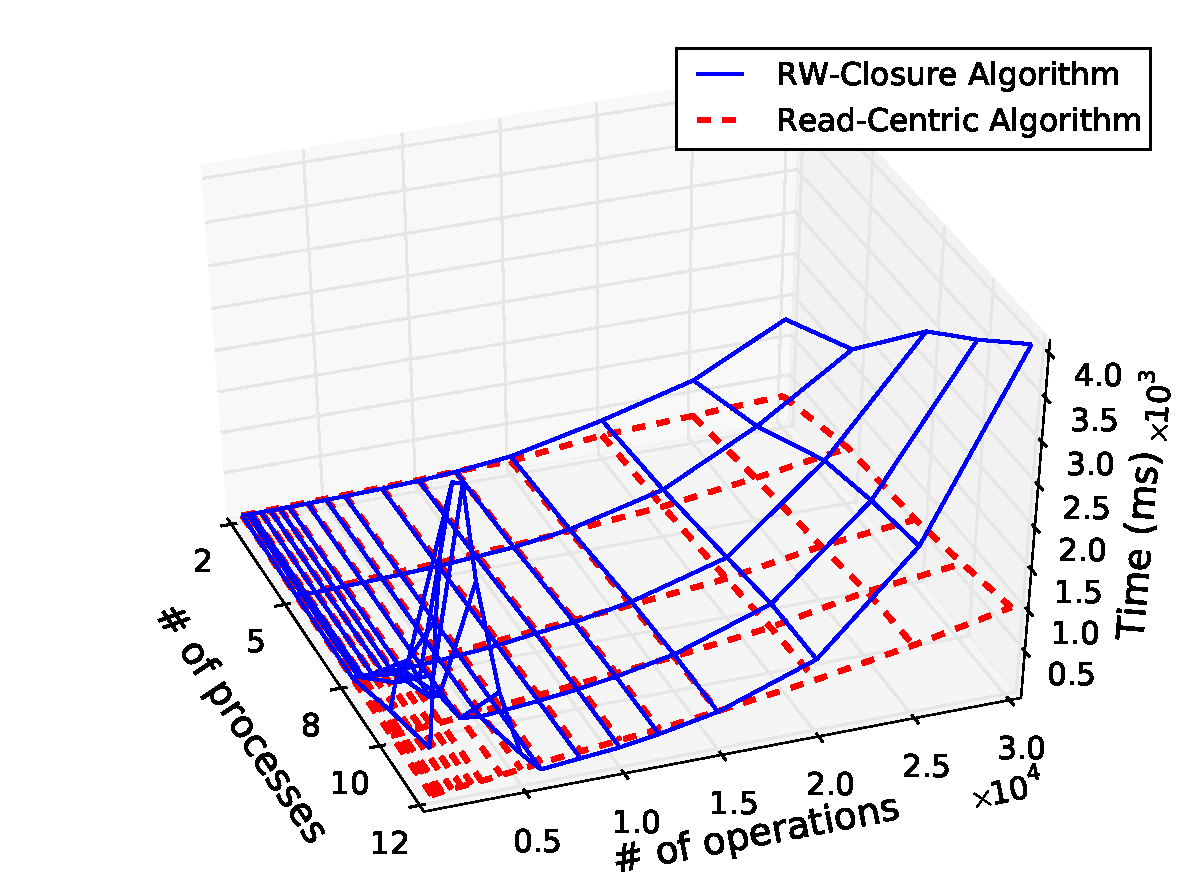
\includegraphics[width = 0.80\textwidth]{figs/vpc-random-cmp.pdf}
    \end{subfigure}%
    ~
    \begin{subfigure}[t]{0.50\textwidth}
      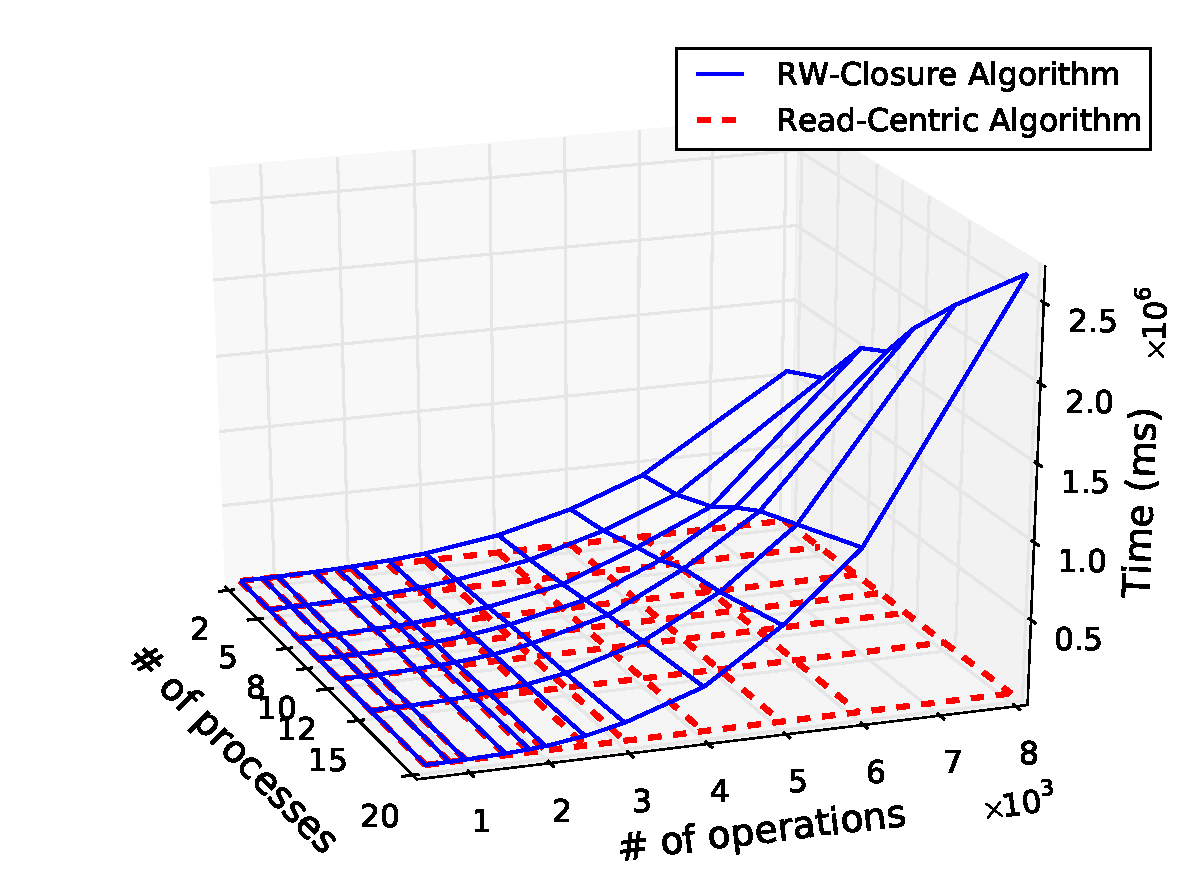
\includegraphics[width = 0.80\textwidth]{figs/vpc-valid-cmp.pdf}
    \end{subfigure}
    \caption{\rwclosure{} 算法与 \readcentric{} 算法在
    \textcolor{blue!80}{ (左) 随机生成}的执行及
    \textcolor{red!80}{ (右) 满足 \PRAM{} 一致性}的执行上的运行时间。}
  \end{figure}

  \pause
  \begin{center}
    \textcolor{red}{(右)} 20个进程、8,000 个操作: 

    \readcentric{} 可获得 694 倍加速.
  \end{center}
\end{frame}
%%%%%%%%%%%%%%%

%%%%%%%%%%%%%%%
\begin{frame}{}
  \fig{width = 0.45\textwidth}{figs/vpc-scalability-more.pdf}
  {\readcentric{} 算法在满足 \PRAM{} 一致性的执行上的运行时间}

  \vspace{-0.30cm}

  \begin{description}
    \centering
    \item[\readcentric{}:] 20个进程、60,000个操作 < 600s~\footnotemark[1]~\footnotetext[1]{用于测试, 规模可用}
    \item[\rwclosure{}:] 20个进程、8,000个操作 > 3,000s
  \end{description}
\end{frame}
%%%%%%%%%%%%%%%
%%%%%%%%%%%%%%%%%%%% End: VPC %%%%%%%%%%%%%%%%%%%%
